\documentclass[spanish]{beamer}

%%% CODIFICACIÓN

%\usepackage[x11names, rgb, html]{xcolor}
\usepackage[utf8]{inputenc}
\usepackage[spanish]{babel}
\usepackage{graphics,tikz}

%%% FUENTES

\usepackage[T1]{fontenc}
\usepackage[familydefault,regular]{Chivo}
\usepackage{newtxsf} % Fuente de matemáticas
\usepackage[scaled=.85]{FiraMono}

\setbeamertemplate{navigation symbols}{}

%%% COLORES

%% Colores de Solarized

\definecolor{sbase03}{HTML}{002B36}
\definecolor{sbase02}{HTML}{073642}
\definecolor{sbase01}{HTML}{586E75}
\definecolor{sbase00}{HTML}{657B83}
\definecolor{sbase0}{HTML}{839496}
\definecolor{sbase1}{HTML}{93A1A1}
\definecolor{sbase2}{HTML}{EEE8D5}
\definecolor{sbase3}{HTML}{FDF6E3}
\definecolor{syellow}{HTML}{B58900}
\definecolor{sorange}{HTML}{CB4B16}
\definecolor{sred}{HTML}{DC322F}
\definecolor{smagenta}{HTML}{D33682}
\definecolor{sviolet}{HTML}{6C71C4}
\definecolor{sblue}{HTML}{268BD2}
\definecolor{scyan}{HTML}{2AA198}
\definecolor{sgreen}{HTML}{859900}

%% Colores del documento

\definecolor{background}{RGB}{237,237,237}
\definecolor{text}{RGB}{78,78,78}
\definecolor{accent}{RGB}{129, 26, 24}
\definecolor{accent2}{HTML}{814918}
\definecolor{accent3}{HTML}{136618}
\definecolor{accent4}{HTML}{0F4B4E}
\definecolor{accent5}{HTML}{681341}
\definecolor{accent6}{HTML}{1F1B5A}

%%% LISTINGS

\usepackage{listingsutf8}

%% Las tildes

\lstset{
  inputencoding=utf8/latin1
}

%% Colores de Solarized para listings

\lstset{
  % How/what to match
  % sensitive=true,
  language=C++,
  % Border (above and below)
  %frame=lines,
  % Line number
  numbers=left,
  % Extra margin on line (align with paragraph)
  xleftmargin=\parindent,
  % Put extra space under caption
  belowcaptionskip=1\baselineskip,
  % Colors
  % backgroundcolor=\color{sbase3},
  basicstyle=\tiny\ttfamily\color{text},
  keywordstyle=\color{accent3},
  commentstyle=\color{accent5},
  stringstyle=\color{accent2},
  numberstyle=\color{text},
  identifierstyle=\color{accent4},
  % Break long lines into multiple lines?
  breaklines=true,
  % Show a character for spaces?
  showstringspaces=false,
  tabsize=2
}

\setbeamerfont{framesubtitle}{size=\normalfont\tiny}
\setbeamercolor{framesubtitle}{fg=white}


%%% AJUSTES DE BEAMER

% ¿Negrita en el título de diapositiva o no?
%\setbeamertemplate{frametitle}{\color{accent}\vspace*{1cm}\bfseries\insertframetitle\par\vskip-6pt}

\setbeamertemplate{frametitle}{\color{accent}\vspace*{1cm}\insertframetitle\par\vskip-6pt}

\setbeamertemplate{itemize items}[circle] % Viñetas de itemize

%%% CONFIGURACIÓN DE COLORES DE BEAMER

\setbeamercolor{background canvas}{bg=background}
\setbeamercolor{normal text}{fg=text}
\setbeamercolor{alerted text}{fg=accent}
\setbeamercolor{block title}{fg=accent}
\setbeamercolor{alerted text}{fg=accent}
\setbeamercolor{itemize item}{fg=accent}
\setbeamercolor{enumerate item}{fg=accent}
\setbeamercolor*{title}{fg=accent}
\setbeamercolor{qed symbol}{fg=accent}
\usebeamercolor[fg]{normal text}

%%% PGFPLOTSTABLE

\usepackage{pgfplotstable}


\pgfplotstableset{
columns/0/.style={
     column name={Elementos},
   },
columns/1/.style={
     column name={Tiempo en segundos},
   },
}

%%% INFORMACIÓN DEL DOCUMENTO

\title{Algorítmica: práctica 2}
\subtitle{Mezclando $k$ vectores ordenados}
\author{Sofía Almeida Bruno\\ Antonio Coín Castro\\ María Victoria Granados Pozo\\ Miguel Lentisco Ballesteros\\ José María Martín Luque\\ \vspace{1em}Grupo 2}
\begin{document}


\maketitle

\begin{frame}{Objetivo}

	\begin{itemize}
		\item Diseño de un algoritmo \textit{divide y vencerás} que se encargue de combinar $k$ vectores ordenados, cada uno con $n$ elementos.
		\item Análisis de su eficiencia teórica, empírica e híbrida.
		\item Comparación con un algoritmo clásico.
	\end{itemize}

\end{frame}

\begin{frame}{Fuerza Bruta}

	Hemos realizado dos algoritmos mediante fuerza bruta:
	\begin{itemize}
		\item Método clásico
		\item Método alternativo
	\end{itemize}
\end{frame}

\begin{frame}{Método Clásico - Mezcla de 2 vectores}
\lstinputlisting[language=C++, linerange={47-70}]{./src/mezcla-vectores-clasico.cpp}
	
\end{frame}

\begin{frame}{Método Clásico}
	\lstinputlisting[language=C++, linerange={75-102}]{./src/mezcla-vectores-clasico.cpp}
\end{frame}

\begin{frame}{Eficiencia teórica}
    \vspace{-1em}
    Consideramos que $n$ es una constante fija.
    
    \vskip 1cm 
	Ecuación general: $$T(k) = \sum_{i=2}^{k-1} ni \thicksim \frac{n}{2}k^2$$
	Orden de eficiencia: $$O\left(\frac{n}{2}k^2\right) \thicksim O(k^2) $$

\end{frame}

\begin{frame}{Eficiencia empírica}
	\begin{center}
		\resizebox*{11cm}{!}{
			% GNUPLOT: LaTeX picture with Postscript
\begingroup
  \makeatletter
  \providecommand\color[2][]{%
    \GenericError{(gnuplot) \space\space\space\@spaces}{%
      Package color not loaded in conjunction with
      terminal option `colourtext'%
    }{See the gnuplot documentation for explanation.%
    }{Either use 'blacktext' in gnuplot or load the package
      color.sty in LaTeX.}%
    \renewcommand\color[2][]{}%
  }%
  \providecommand\includegraphics[2][]{%
    \GenericError{(gnuplot) \space\space\space\@spaces}{%
      Package graphicx or graphics not loaded%
    }{See the gnuplot documentation for explanation.%
    }{The gnuplot epslatex terminal needs graphicx.sty or graphics.sty.}%
    \renewcommand\includegraphics[2][]{}%
  }%
  \providecommand\rotatebox[2]{#2}%
  \@ifundefined{ifGPcolor}{%
    \newif\ifGPcolor
    \GPcolortrue
  }{}%
  \@ifundefined{ifGPblacktext}{%
    \newif\ifGPblacktext
    \GPblacktextfalse
  }{}%
  % define a \g@addto@macro without @ in the name:
  \let\gplgaddtomacro\g@addto@macro
  % define empty templates for all commands taking text:
  \gdef\gplbacktext{}%
  \gdef\gplfronttext{}%
  \makeatother
  \ifGPblacktext
    % no textcolor at all
    \def\colorrgb#1{}%
    \def\colorgray#1{}%
  \else
    % gray or color?
    \ifGPcolor
      \def\colorrgb#1{\color[rgb]{#1}}%
      \def\colorgray#1{\color[gray]{#1}}%
      \expandafter\def\csname LTw\endcsname{\color{white}}%
      \expandafter\def\csname LTb\endcsname{\color{black}}%
      \expandafter\def\csname LTa\endcsname{\color{black}}%
      \expandafter\def\csname LT0\endcsname{\color[rgb]{1,0,0}}%
      \expandafter\def\csname LT1\endcsname{\color[rgb]{0,1,0}}%
      \expandafter\def\csname LT2\endcsname{\color[rgb]{0,0,1}}%
      \expandafter\def\csname LT3\endcsname{\color[rgb]{1,0,1}}%
      \expandafter\def\csname LT4\endcsname{\color[rgb]{0,1,1}}%
      \expandafter\def\csname LT5\endcsname{\color[rgb]{1,1,0}}%
      \expandafter\def\csname LT6\endcsname{\color[rgb]{0,0,0}}%
      \expandafter\def\csname LT7\endcsname{\color[rgb]{1,0.3,0}}%
      \expandafter\def\csname LT8\endcsname{\color[rgb]{0.5,0.5,0.5}}%
    \else
      % gray
      \def\colorrgb#1{\color{black}}%
      \def\colorgray#1{\color[gray]{#1}}%
      \expandafter\def\csname LTw\endcsname{\color{white}}%
      \expandafter\def\csname LTb\endcsname{\color{black}}%
      \expandafter\def\csname LTa\endcsname{\color{black}}%
      \expandafter\def\csname LT0\endcsname{\color{black}}%
      \expandafter\def\csname LT1\endcsname{\color{black}}%
      \expandafter\def\csname LT2\endcsname{\color{black}}%
      \expandafter\def\csname LT3\endcsname{\color{black}}%
      \expandafter\def\csname LT4\endcsname{\color{black}}%
      \expandafter\def\csname LT5\endcsname{\color{black}}%
      \expandafter\def\csname LT6\endcsname{\color{black}}%
      \expandafter\def\csname LT7\endcsname{\color{black}}%
      \expandafter\def\csname LT8\endcsname{\color{black}}%
    \fi
  \fi
    \setlength{\unitlength}{0.0500bp}%
    \ifx\gptboxheight\undefined%
      \newlength{\gptboxheight}%
      \newlength{\gptboxwidth}%
      \newsavebox{\gptboxtext}%
    \fi%
    \setlength{\fboxrule}{0.5pt}%
    \setlength{\fboxsep}{1pt}%
\begin{picture}(7200.00,4320.00)%
    \gplgaddtomacro\gplbacktext{%
      \colorrgb{0.30,0.30,0.30}%
      \put(1386,1060){\makebox(0,0)[r]{\strut{}$\textcolor{text}{0}$}}%
      \colorrgb{0.30,0.30,0.30}%
      \put(1386,1349){\makebox(0,0)[r]{\strut{}$\textcolor{text}{0.05}$}}%
      \colorrgb{0.30,0.30,0.30}%
      \put(1386,1638){\makebox(0,0)[r]{\strut{}$\textcolor{text}{0.1}$}}%
      \colorrgb{0.30,0.30,0.30}%
      \put(1386,1926){\makebox(0,0)[r]{\strut{}$\textcolor{text}{0.15}$}}%
      \colorrgb{0.30,0.30,0.30}%
      \put(1386,2215){\makebox(0,0)[r]{\strut{}$\textcolor{text}{0.2}$}}%
      \colorrgb{0.30,0.30,0.30}%
      \put(1386,2504){\makebox(0,0)[r]{\strut{}$\textcolor{text}{0.25}$}}%
      \colorrgb{0.30,0.30,0.30}%
      \put(1386,2793){\makebox(0,0)[r]{\strut{}$\textcolor{text}{0.3}$}}%
      \colorrgb{0.30,0.30,0.30}%
      \put(1386,3081){\makebox(0,0)[r]{\strut{}$\textcolor{text}{0.35}$}}%
      \colorrgb{0.30,0.30,0.30}%
      \put(1386,3370){\makebox(0,0)[r]{\strut{}$\textcolor{text}{0.4}$}}%
      \colorrgb{0.30,0.30,0.30}%
      \put(1386,3659){\makebox(0,0)[r]{\strut{}$\textcolor{text}{0.45}$}}%
      \colorrgb{0.30,0.30,0.30}%
      \put(1518,928){\rotatebox{45}{\makebox(0,0)[r]{\strut{}$\textcolor{text}{0}$}}}%
      \colorrgb{0.30,0.30,0.30}%
      \put(2047,928){\rotatebox{45}{\makebox(0,0)[r]{\strut{}$\textcolor{text}{500}$}}}%
      \colorrgb{0.30,0.30,0.30}%
      \put(2575,928){\rotatebox{45}{\makebox(0,0)[r]{\strut{}$\textcolor{text}{1000}$}}}%
      \colorrgb{0.30,0.30,0.30}%
      \put(3104,928){\rotatebox{45}{\makebox(0,0)[r]{\strut{}$\textcolor{text}{1500}$}}}%
      \colorrgb{0.30,0.30,0.30}%
      \put(3632,928){\rotatebox{45}{\makebox(0,0)[r]{\strut{}$\textcolor{text}{2000}$}}}%
      \colorrgb{0.30,0.30,0.30}%
      \put(4161,928){\rotatebox{45}{\makebox(0,0)[r]{\strut{}$\textcolor{text}{2500}$}}}%
      \colorrgb{0.30,0.30,0.30}%
      \put(4689,928){\rotatebox{45}{\makebox(0,0)[r]{\strut{}$\textcolor{text}{3000}$}}}%
      \colorrgb{0.30,0.30,0.30}%
      \put(5218,928){\rotatebox{45}{\makebox(0,0)[r]{\strut{}$\textcolor{text}{3500}$}}}%
      \colorrgb{0.30,0.30,0.30}%
      \put(5746,928){\rotatebox{45}{\makebox(0,0)[r]{\strut{}$\textcolor{text}{4000}$}}}%
      \colorrgb{0.30,0.30,0.30}%
      \put(6275,928){\rotatebox{45}{\makebox(0,0)[r]{\strut{}$\textcolor{text}{4500}$}}}%
      \colorrgb{0.30,0.30,0.30}%
      \put(6803,928){\rotatebox{45}{\makebox(0,0)[r]{\strut{}$\textcolor{text}{5000}$}}}%
    }%
    \gplgaddtomacro\gplfronttext{%
      \colorrgb{0.30,0.30,0.30}%
      \put(220,2359){\rotatebox{-270}{\makebox(0,0){\strut{}Tiempo de ejecución (s)}}}%
      \colorrgb{0.30,0.30,0.30}%
      \put(4160,220){\makebox(0,0){\strut{}Número de vectores (k)}}%
      \colorrgb{0.30,0.30,0.30}%
      \put(4160,3989){\makebox(0,0){\strut{}Eficiencia empírica mezcla-vectores-clasico}}%
      \csname LTb\endcsname%
      \put(5816,3486){\makebox(0,0)[r]{\strut{}Algoritmo divide y vencerás n = 10}}%
    }%
    \gplbacktext
    \put(0,0){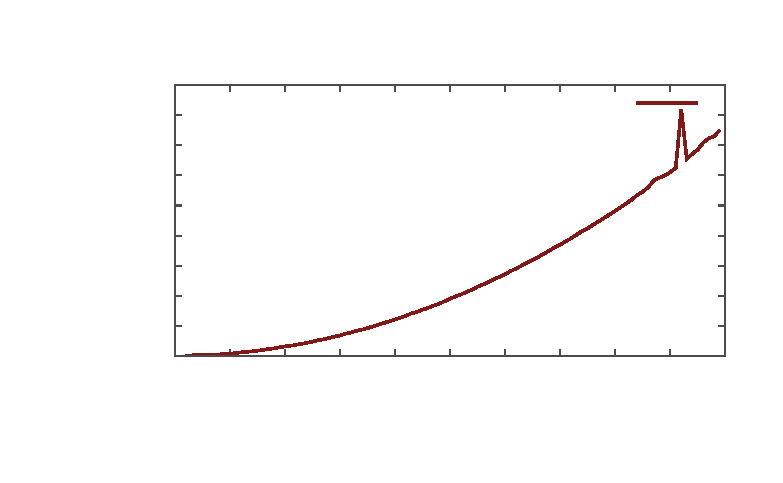
\includegraphics{graficos/mezcla-vectores-clasico}}%
    \gplfronttext
  \end{picture}%
\endgroup
}
	\end{center}

\end{frame}

\begin{frame}{Eficiencia híbrida}
  \fontsize{8pt}{7.2}\selectfont
	\begin{center}
	\resizebox*{11cm}{!}{
		% GNUPLOT: LaTeX picture with Postscript
\begingroup
  \makeatletter
  \providecommand\color[2][]{%
    \GenericError{(gnuplot) \space\space\space\@spaces}{%
      Package color not loaded in conjunction with
      terminal option `colourtext'%
    }{See the gnuplot documentation for explanation.%
    }{Either use 'blacktext' in gnuplot or load the package
      color.sty in LaTeX.}%
    \renewcommand\color[2][]{}%
  }%
  \providecommand\includegraphics[2][]{%
    \GenericError{(gnuplot) \space\space\space\@spaces}{%
      Package graphicx or graphics not loaded%
    }{See the gnuplot documentation for explanation.%
    }{The gnuplot epslatex terminal needs graphicx.sty or graphics.sty.}%
    \renewcommand\includegraphics[2][]{}%
  }%
  \providecommand\rotatebox[2]{#2}%
  \@ifundefined{ifGPcolor}{%
    \newif\ifGPcolor
    \GPcolortrue
  }{}%
  \@ifundefined{ifGPblacktext}{%
    \newif\ifGPblacktext
    \GPblacktextfalse
  }{}%
  % define a \g@addto@macro without @ in the name:
  \let\gplgaddtomacro\g@addto@macro
  % define empty templates for all commands taking text:
  \gdef\gplbacktext{}%
  \gdef\gplfronttext{}%
  \makeatother
  \ifGPblacktext
    % no textcolor at all
    \def\colorrgb#1{}%
    \def\colorgray#1{}%
  \else
    % gray or color?
    \ifGPcolor
      \def\colorrgb#1{\color[rgb]{#1}}%
      \def\colorgray#1{\color[gray]{#1}}%
      \expandafter\def\csname LTw\endcsname{\color{white}}%
      \expandafter\def\csname LTb\endcsname{\color{black}}%
      \expandafter\def\csname LTa\endcsname{\color{black}}%
      \expandafter\def\csname LT0\endcsname{\color[rgb]{1,0,0}}%
      \expandafter\def\csname LT1\endcsname{\color[rgb]{0,1,0}}%
      \expandafter\def\csname LT2\endcsname{\color[rgb]{0,0,1}}%
      \expandafter\def\csname LT3\endcsname{\color[rgb]{1,0,1}}%
      \expandafter\def\csname LT4\endcsname{\color[rgb]{0,1,1}}%
      \expandafter\def\csname LT5\endcsname{\color[rgb]{1,1,0}}%
      \expandafter\def\csname LT6\endcsname{\color[rgb]{0,0,0}}%
      \expandafter\def\csname LT7\endcsname{\color[rgb]{1,0.3,0}}%
      \expandafter\def\csname LT8\endcsname{\color[rgb]{0.5,0.5,0.5}}%
    \else
      % gray
      \def\colorrgb#1{\color{black}}%
      \def\colorgray#1{\color[gray]{#1}}%
      \expandafter\def\csname LTw\endcsname{\color{white}}%
      \expandafter\def\csname LTb\endcsname{\color{black}}%
      \expandafter\def\csname LTa\endcsname{\color{black}}%
      \expandafter\def\csname LT0\endcsname{\color{black}}%
      \expandafter\def\csname LT1\endcsname{\color{black}}%
      \expandafter\def\csname LT2\endcsname{\color{black}}%
      \expandafter\def\csname LT3\endcsname{\color{black}}%
      \expandafter\def\csname LT4\endcsname{\color{black}}%
      \expandafter\def\csname LT5\endcsname{\color{black}}%
      \expandafter\def\csname LT6\endcsname{\color{black}}%
      \expandafter\def\csname LT7\endcsname{\color{black}}%
      \expandafter\def\csname LT8\endcsname{\color{black}}%
    \fi
  \fi
    \setlength{\unitlength}{0.0500bp}%
    \ifx\gptboxheight\undefined%
      \newlength{\gptboxheight}%
      \newlength{\gptboxwidth}%
      \newsavebox{\gptboxtext}%
    \fi%
    \setlength{\fboxrule}{0.5pt}%
    \setlength{\fboxsep}{1pt}%
\begin{picture}(5760.00,4320.00)%
    \gplgaddtomacro\gplbacktext{%
      \colorrgb{0.30,0.30,0.30}%
      \put(1386,1060){\makebox(0,0)[r]{\strut{}$\textcolor{text}{0}$}}%
      \colorrgb{0.30,0.30,0.30}%
      \put(1386,1349){\makebox(0,0)[r]{\strut{}$\textcolor{text}{0.05}$}}%
      \colorrgb{0.30,0.30,0.30}%
      \put(1386,1638){\makebox(0,0)[r]{\strut{}$\textcolor{text}{0.1}$}}%
      \colorrgb{0.30,0.30,0.30}%
      \put(1386,1926){\makebox(0,0)[r]{\strut{}$\textcolor{text}{0.15}$}}%
      \colorrgb{0.30,0.30,0.30}%
      \put(1386,2215){\makebox(0,0)[r]{\strut{}$\textcolor{text}{0.2}$}}%
      \colorrgb{0.30,0.30,0.30}%
      \put(1386,2504){\makebox(0,0)[r]{\strut{}$\textcolor{text}{0.25}$}}%
      \colorrgb{0.30,0.30,0.30}%
      \put(1386,2793){\makebox(0,0)[r]{\strut{}$\textcolor{text}{0.3}$}}%
      \colorrgb{0.30,0.30,0.30}%
      \put(1386,3081){\makebox(0,0)[r]{\strut{}$\textcolor{text}{0.35}$}}%
      \colorrgb{0.30,0.30,0.30}%
      \put(1386,3370){\makebox(0,0)[r]{\strut{}$\textcolor{text}{0.4}$}}%
      \colorrgb{0.30,0.30,0.30}%
      \put(1386,3659){\makebox(0,0)[r]{\strut{}$\textcolor{text}{0.45}$}}%
      \colorrgb{0.30,0.30,0.30}%
      \put(1518,928){\rotatebox{45}{\makebox(0,0)[r]{\strut{}$\textcolor{text}{0}$}}}%
      \colorrgb{0.30,0.30,0.30}%
      \put(1903,928){\rotatebox{45}{\makebox(0,0)[r]{\strut{}$\textcolor{text}{500}$}}}%
      \colorrgb{0.30,0.30,0.30}%
      \put(2287,928){\rotatebox{45}{\makebox(0,0)[r]{\strut{}$\textcolor{text}{1000}$}}}%
      \colorrgb{0.30,0.30,0.30}%
      \put(2672,928){\rotatebox{45}{\makebox(0,0)[r]{\strut{}$\textcolor{text}{1500}$}}}%
      \colorrgb{0.30,0.30,0.30}%
      \put(3056,928){\rotatebox{45}{\makebox(0,0)[r]{\strut{}$\textcolor{text}{2000}$}}}%
      \colorrgb{0.30,0.30,0.30}%
      \put(3441,928){\rotatebox{45}{\makebox(0,0)[r]{\strut{}$\textcolor{text}{2500}$}}}%
      \colorrgb{0.30,0.30,0.30}%
      \put(3825,928){\rotatebox{45}{\makebox(0,0)[r]{\strut{}$\textcolor{text}{3000}$}}}%
      \colorrgb{0.30,0.30,0.30}%
      \put(4210,928){\rotatebox{45}{\makebox(0,0)[r]{\strut{}$\textcolor{text}{3500}$}}}%
      \colorrgb{0.30,0.30,0.30}%
      \put(4594,928){\rotatebox{45}{\makebox(0,0)[r]{\strut{}$\textcolor{text}{4000}$}}}%
      \colorrgb{0.30,0.30,0.30}%
      \put(4979,928){\rotatebox{45}{\makebox(0,0)[r]{\strut{}$\textcolor{text}{4500}$}}}%
      \colorrgb{0.30,0.30,0.30}%
      \put(5363,928){\rotatebox{45}{\makebox(0,0)[r]{\strut{}$\textcolor{text}{5000}$}}}%
    }%
    \gplgaddtomacro\gplfronttext{%
      \colorrgb{0.30,0.30,0.30}%
      \put(220,2359){\rotatebox{-270}{\makebox(0,0){\strut{}Tiempo de ejecución (s)}}}%
      \colorrgb{0.30,0.30,0.30}%
      \put(3440,220){\makebox(0,0){\strut{}Tamaño del vector (elementos)}}%
      \colorrgb{0.30,0.30,0.30}%
      \put(3440,3989){\makebox(0,0){\strut{}Ajuste algoritmo clásico}}%
      \csname LTb\endcsname%
      \put(4376,3486){\makebox(0,0)[r]{\strut{}3.22e-09$x^2$+-3.73e-06$x$+2.57e-03}}%
      \csname LTb\endcsname%
      \put(4376,3266){\makebox(0,0)[r]{\strut{}Clásico}}%
    }%
    \gplbacktext
    \put(0,0){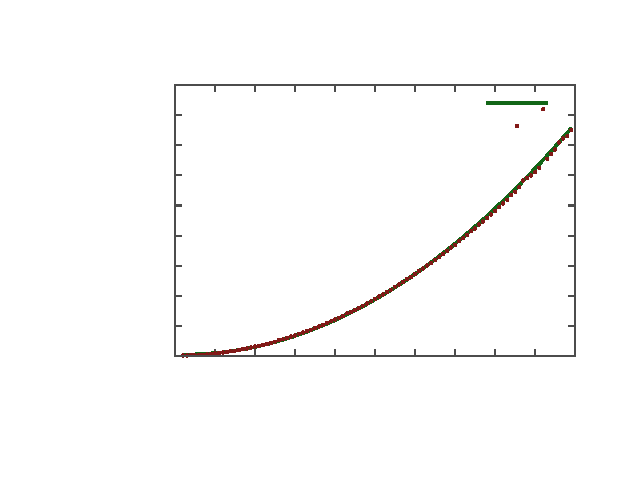
\includegraphics{./graficos/ajuste-clasico}}%
    \gplfronttext
  \end{picture}%
\endgroup

	}
	\end{center}
\end{frame}

\begin{frame}{Método Alternativo}
	\lstinputlisting[language=C++, linerange={12-39}]{./src/mezcla-vectores-clasico-v2.cpp}
\end{frame}

\begin{frame}{Eficiencia empírica}
	\begin{center}
		\resizebox*{11cm}{!}{
			% GNUPLOT: LaTeX picture with Postscript
\begingroup
  \makeatletter
  \providecommand\color[2][]{%
    \GenericError{(gnuplot) \space\space\space\@spaces}{%
      Package color not loaded in conjunction with
      terminal option `colourtext'%
    }{See the gnuplot documentation for explanation.%
    }{Either use 'blacktext' in gnuplot or load the package
      color.sty in LaTeX.}%
    \renewcommand\color[2][]{}%
  }%
  \providecommand\includegraphics[2][]{%
    \GenericError{(gnuplot) \space\space\space\@spaces}{%
      Package graphicx or graphics not loaded%
    }{See the gnuplot documentation for explanation.%
    }{The gnuplot epslatex terminal needs graphicx.sty or graphics.sty.}%
    \renewcommand\includegraphics[2][]{}%
  }%
  \providecommand\rotatebox[2]{#2}%
  \@ifundefined{ifGPcolor}{%
    \newif\ifGPcolor
    \GPcolortrue
  }{}%
  \@ifundefined{ifGPblacktext}{%
    \newif\ifGPblacktext
    \GPblacktextfalse
  }{}%
  % define a \g@addto@macro without @ in the name:
  \let\gplgaddtomacro\g@addto@macro
  % define empty templates for all commands taking text:
  \gdef\gplbacktext{}%
  \gdef\gplfronttext{}%
  \makeatother
  \ifGPblacktext
    % no textcolor at all
    \def\colorrgb#1{}%
    \def\colorgray#1{}%
  \else
    % gray or color?
    \ifGPcolor
      \def\colorrgb#1{\color[rgb]{#1}}%
      \def\colorgray#1{\color[gray]{#1}}%
      \expandafter\def\csname LTw\endcsname{\color{white}}%
      \expandafter\def\csname LTb\endcsname{\color{black}}%
      \expandafter\def\csname LTa\endcsname{\color{black}}%
      \expandafter\def\csname LT0\endcsname{\color[rgb]{1,0,0}}%
      \expandafter\def\csname LT1\endcsname{\color[rgb]{0,1,0}}%
      \expandafter\def\csname LT2\endcsname{\color[rgb]{0,0,1}}%
      \expandafter\def\csname LT3\endcsname{\color[rgb]{1,0,1}}%
      \expandafter\def\csname LT4\endcsname{\color[rgb]{0,1,1}}%
      \expandafter\def\csname LT5\endcsname{\color[rgb]{1,1,0}}%
      \expandafter\def\csname LT6\endcsname{\color[rgb]{0,0,0}}%
      \expandafter\def\csname LT7\endcsname{\color[rgb]{1,0.3,0}}%
      \expandafter\def\csname LT8\endcsname{\color[rgb]{0.5,0.5,0.5}}%
    \else
      % gray
      \def\colorrgb#1{\color{black}}%
      \def\colorgray#1{\color[gray]{#1}}%
      \expandafter\def\csname LTw\endcsname{\color{white}}%
      \expandafter\def\csname LTb\endcsname{\color{black}}%
      \expandafter\def\csname LTa\endcsname{\color{black}}%
      \expandafter\def\csname LT0\endcsname{\color{black}}%
      \expandafter\def\csname LT1\endcsname{\color{black}}%
      \expandafter\def\csname LT2\endcsname{\color{black}}%
      \expandafter\def\csname LT3\endcsname{\color{black}}%
      \expandafter\def\csname LT4\endcsname{\color{black}}%
      \expandafter\def\csname LT5\endcsname{\color{black}}%
      \expandafter\def\csname LT6\endcsname{\color{black}}%
      \expandafter\def\csname LT7\endcsname{\color{black}}%
      \expandafter\def\csname LT8\endcsname{\color{black}}%
    \fi
  \fi
  \setlength{\unitlength}{0.0500bp}%
  \begin{picture}(7200.00,4320.00)%
    \gplgaddtomacro\gplbacktext{%
      \colorrgb{0.30,0.30,0.30}%
      \put(1474,1324){\makebox(0,0)[r]{\strut{}$\textcolor{text}{0}$}}%
      \colorrgb{0.30,0.30,0.30}%
      \put(1474,1583){\makebox(0,0)[r]{\strut{}$\textcolor{text}{0.1}$}}%
      \colorrgb{0.30,0.30,0.30}%
      \put(1474,1843){\makebox(0,0)[r]{\strut{}$\textcolor{text}{0.2}$}}%
      \colorrgb{0.30,0.30,0.30}%
      \put(1474,2102){\makebox(0,0)[r]{\strut{}$\textcolor{text}{0.3}$}}%
      \colorrgb{0.30,0.30,0.30}%
      \put(1474,2362){\makebox(0,0)[r]{\strut{}$\textcolor{text}{0.4}$}}%
      \colorrgb{0.30,0.30,0.30}%
      \put(1474,2621){\makebox(0,0)[r]{\strut{}$\textcolor{text}{0.5}$}}%
      \colorrgb{0.30,0.30,0.30}%
      \put(1474,2881){\makebox(0,0)[r]{\strut{}$\textcolor{text}{0.6}$}}%
      \colorrgb{0.30,0.30,0.30}%
      \put(1474,3140){\makebox(0,0)[r]{\strut{}$\textcolor{text}{0.7}$}}%
      \colorrgb{0.30,0.30,0.30}%
      \put(1474,3400){\makebox(0,0)[r]{\strut{}$\textcolor{text}{0.8}$}}%
      \colorrgb{0.30,0.30,0.30}%
      \put(1474,3659){\makebox(0,0)[r]{\strut{}$\textcolor{text}{0.9}$}}%
      \colorrgb{0.30,0.30,0.30}%
      \put(1606,1192){\rotatebox{45}{\makebox(0,0)[r]{\strut{}$\textcolor{text}{0}$}}}%
      \colorrgb{0.30,0.30,0.30}%
      \put(2126,1192){\rotatebox{45}{\makebox(0,0)[r]{\strut{}$\textcolor{text}{500}$}}}%
      \colorrgb{0.30,0.30,0.30}%
      \put(2645,1192){\rotatebox{45}{\makebox(0,0)[r]{\strut{}$\textcolor{text}{1000}$}}}%
      \colorrgb{0.30,0.30,0.30}%
      \put(3165,1192){\rotatebox{45}{\makebox(0,0)[r]{\strut{}$\textcolor{text}{1500}$}}}%
      \colorrgb{0.30,0.30,0.30}%
      \put(3685,1192){\rotatebox{45}{\makebox(0,0)[r]{\strut{}$\textcolor{text}{2000}$}}}%
      \colorrgb{0.30,0.30,0.30}%
      \put(4205,1192){\rotatebox{45}{\makebox(0,0)[r]{\strut{}$\textcolor{text}{2500}$}}}%
      \colorrgb{0.30,0.30,0.30}%
      \put(4724,1192){\rotatebox{45}{\makebox(0,0)[r]{\strut{}$\textcolor{text}{3000}$}}}%
      \colorrgb{0.30,0.30,0.30}%
      \put(5244,1192){\rotatebox{45}{\makebox(0,0)[r]{\strut{}$\textcolor{text}{3500}$}}}%
      \colorrgb{0.30,0.30,0.30}%
      \put(5764,1192){\rotatebox{45}{\makebox(0,0)[r]{\strut{}$\textcolor{text}{4000}$}}}%
      \colorrgb{0.30,0.30,0.30}%
      \put(6283,1192){\rotatebox{45}{\makebox(0,0)[r]{\strut{}$\textcolor{text}{4500}$}}}%
      \colorrgb{0.30,0.30,0.30}%
      \put(6803,1192){\rotatebox{45}{\makebox(0,0)[r]{\strut{}$\textcolor{text}{5000}$}}}%
      \csname LTb\endcsname%
      \put(176,2491){\rotatebox{-270}{\makebox(0,0){\strut{}Tiempo de ejecución (s)}}}%
      \put(4204,154){\makebox(0,0){\strut{}Número de vectores (k)}}%
      \put(4204,3989){\makebox(0,0){\strut{}Eficiencia empírica mezcla-vectores-clasico-v2}}%
    }%
    \gplgaddtomacro\gplfronttext{%
      \csname LTb\endcsname%
      \put(5816,3486){\makebox(0,0)[r]{\strut{}Algoritmo clásico n = 10}}%
    }%
    \gplbacktext
    \put(0,0){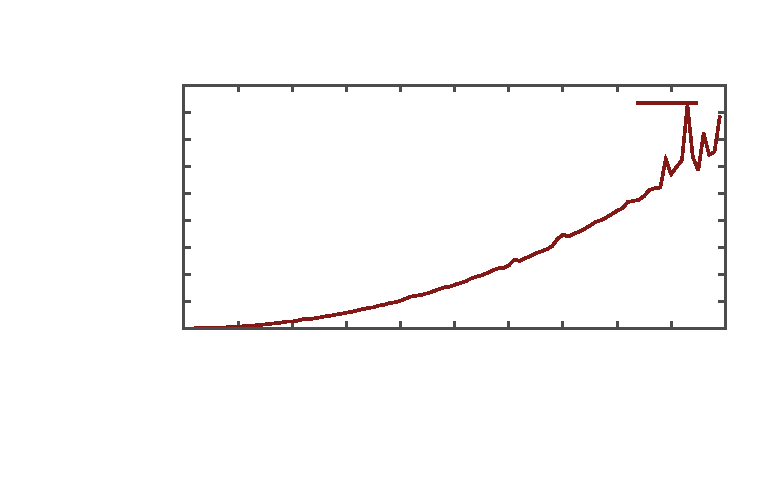
\includegraphics{graficos/mezcla-vectores-clasico-v2}}%
    \gplfronttext
  \end{picture}%
\endgroup
}
	\end{center}
\end{frame}

\begin{frame}{Eficiencia híbrida}
  \fontsize{8pt}{7.2}\selectfont
	\begin{center}
	\resizebox*{11cm}{!}{
		% GNUPLOT: LaTeX picture with Postscript
\begingroup
  \makeatletter
  \providecommand\color[2][]{%
    \GenericError{(gnuplot) \space\space\space\@spaces}{%
      Package color not loaded in conjunction with
      terminal option `colourtext'%
    }{See the gnuplot documentation for explanation.%
    }{Either use 'blacktext' in gnuplot or load the package
      color.sty in LaTeX.}%
    \renewcommand\color[2][]{}%
  }%
  \providecommand\includegraphics[2][]{%
    \GenericError{(gnuplot) \space\space\space\@spaces}{%
      Package graphicx or graphics not loaded%
    }{See the gnuplot documentation for explanation.%
    }{The gnuplot epslatex terminal needs graphicx.sty or graphics.sty.}%
    \renewcommand\includegraphics[2][]{}%
  }%
  \providecommand\rotatebox[2]{#2}%
  \@ifundefined{ifGPcolor}{%
    \newif\ifGPcolor
    \GPcolortrue
  }{}%
  \@ifundefined{ifGPblacktext}{%
    \newif\ifGPblacktext
    \GPblacktextfalse
  }{}%
  % define a \g@addto@macro without @ in the name:
  \let\gplgaddtomacro\g@addto@macro
  % define empty templates for all commands taking text:
  \gdef\gplbacktext{}%
  \gdef\gplfronttext{}%
  \makeatother
  \ifGPblacktext
    % no textcolor at all
    \def\colorrgb#1{}%
    \def\colorgray#1{}%
  \else
    % gray or color?
    \ifGPcolor
      \def\colorrgb#1{\color[rgb]{#1}}%
      \def\colorgray#1{\color[gray]{#1}}%
      \expandafter\def\csname LTw\endcsname{\color{white}}%
      \expandafter\def\csname LTb\endcsname{\color{black}}%
      \expandafter\def\csname LTa\endcsname{\color{black}}%
      \expandafter\def\csname LT0\endcsname{\color[rgb]{1,0,0}}%
      \expandafter\def\csname LT1\endcsname{\color[rgb]{0,1,0}}%
      \expandafter\def\csname LT2\endcsname{\color[rgb]{0,0,1}}%
      \expandafter\def\csname LT3\endcsname{\color[rgb]{1,0,1}}%
      \expandafter\def\csname LT4\endcsname{\color[rgb]{0,1,1}}%
      \expandafter\def\csname LT5\endcsname{\color[rgb]{1,1,0}}%
      \expandafter\def\csname LT6\endcsname{\color[rgb]{0,0,0}}%
      \expandafter\def\csname LT7\endcsname{\color[rgb]{1,0.3,0}}%
      \expandafter\def\csname LT8\endcsname{\color[rgb]{0.5,0.5,0.5}}%
    \else
      % gray
      \def\colorrgb#1{\color{black}}%
      \def\colorgray#1{\color[gray]{#1}}%
      \expandafter\def\csname LTw\endcsname{\color{white}}%
      \expandafter\def\csname LTb\endcsname{\color{black}}%
      \expandafter\def\csname LTa\endcsname{\color{black}}%
      \expandafter\def\csname LT0\endcsname{\color{black}}%
      \expandafter\def\csname LT1\endcsname{\color{black}}%
      \expandafter\def\csname LT2\endcsname{\color{black}}%
      \expandafter\def\csname LT3\endcsname{\color{black}}%
      \expandafter\def\csname LT4\endcsname{\color{black}}%
      \expandafter\def\csname LT5\endcsname{\color{black}}%
      \expandafter\def\csname LT6\endcsname{\color{black}}%
      \expandafter\def\csname LT7\endcsname{\color{black}}%
      \expandafter\def\csname LT8\endcsname{\color{black}}%
    \fi
  \fi
  \setlength{\unitlength}{0.0500bp}%
  \begin{picture}(5760.00,4320.00)%
    \gplgaddtomacro\gplbacktext{%
      \colorrgb{0.30,0.30,0.30}%
      \put(1474,1324){\makebox(0,0)[r]{\strut{}$\textcolor{text}{0}$}}%
      \colorrgb{0.30,0.30,0.30}%
      \put(1474,1583){\makebox(0,0)[r]{\strut{}$\textcolor{text}{0.1}$}}%
      \colorrgb{0.30,0.30,0.30}%
      \put(1474,1843){\makebox(0,0)[r]{\strut{}$\textcolor{text}{0.2}$}}%
      \colorrgb{0.30,0.30,0.30}%
      \put(1474,2102){\makebox(0,0)[r]{\strut{}$\textcolor{text}{0.3}$}}%
      \colorrgb{0.30,0.30,0.30}%
      \put(1474,2362){\makebox(0,0)[r]{\strut{}$\textcolor{text}{0.4}$}}%
      \colorrgb{0.30,0.30,0.30}%
      \put(1474,2621){\makebox(0,0)[r]{\strut{}$\textcolor{text}{0.5}$}}%
      \colorrgb{0.30,0.30,0.30}%
      \put(1474,2881){\makebox(0,0)[r]{\strut{}$\textcolor{text}{0.6}$}}%
      \colorrgb{0.30,0.30,0.30}%
      \put(1474,3140){\makebox(0,0)[r]{\strut{}$\textcolor{text}{0.7}$}}%
      \colorrgb{0.30,0.30,0.30}%
      \put(1474,3400){\makebox(0,0)[r]{\strut{}$\textcolor{text}{0.8}$}}%
      \colorrgb{0.30,0.30,0.30}%
      \put(1474,3659){\makebox(0,0)[r]{\strut{}$\textcolor{text}{0.9}$}}%
      \colorrgb{0.30,0.30,0.30}%
      \put(1606,1192){\rotatebox{45}{\makebox(0,0)[r]{\strut{}$\textcolor{text}{0}$}}}%
      \colorrgb{0.30,0.30,0.30}%
      \put(1982,1192){\rotatebox{45}{\makebox(0,0)[r]{\strut{}$\textcolor{text}{500}$}}}%
      \colorrgb{0.30,0.30,0.30}%
      \put(2357,1192){\rotatebox{45}{\makebox(0,0)[r]{\strut{}$\textcolor{text}{1000}$}}}%
      \colorrgb{0.30,0.30,0.30}%
      \put(2733,1192){\rotatebox{45}{\makebox(0,0)[r]{\strut{}$\textcolor{text}{1500}$}}}%
      \colorrgb{0.30,0.30,0.30}%
      \put(3109,1192){\rotatebox{45}{\makebox(0,0)[r]{\strut{}$\textcolor{text}{2000}$}}}%
      \colorrgb{0.30,0.30,0.30}%
      \put(3485,1192){\rotatebox{45}{\makebox(0,0)[r]{\strut{}$\textcolor{text}{2500}$}}}%
      \colorrgb{0.30,0.30,0.30}%
      \put(3860,1192){\rotatebox{45}{\makebox(0,0)[r]{\strut{}$\textcolor{text}{3000}$}}}%
      \colorrgb{0.30,0.30,0.30}%
      \put(4236,1192){\rotatebox{45}{\makebox(0,0)[r]{\strut{}$\textcolor{text}{3500}$}}}%
      \colorrgb{0.30,0.30,0.30}%
      \put(4612,1192){\rotatebox{45}{\makebox(0,0)[r]{\strut{}$\textcolor{text}{4000}$}}}%
      \colorrgb{0.30,0.30,0.30}%
      \put(4987,1192){\rotatebox{45}{\makebox(0,0)[r]{\strut{}$\textcolor{text}{4500}$}}}%
      \colorrgb{0.30,0.30,0.30}%
      \put(5363,1192){\rotatebox{45}{\makebox(0,0)[r]{\strut{}$\textcolor{text}{5000}$}}}%
      \csname LTb\endcsname%
      \put(176,2491){\rotatebox{-270}{\makebox(0,0){\strut{}Tiempo de ejecución (s)}}}%
      \put(3484,154){\makebox(0,0){\strut{}Tamaño del vector (elementos)}}%
      \put(3484,3989){\makebox(0,0){\strut{}Ajuste algoritmo clásico - v2}}%
    }%
    \gplgaddtomacro\gplfronttext{%
      \csname LTb\endcsname%
      \put(4376,3486){\makebox(0,0)[r]{\strut{}6.87e-09$x^2$+-2.88e-05$x$+1.69e-02}}%
      \csname LTb\endcsname%
      \put(4376,3266){\makebox(0,0)[r]{\strut{}Clásico - v2}}%
    }%
    \gplbacktext
    \put(0,0){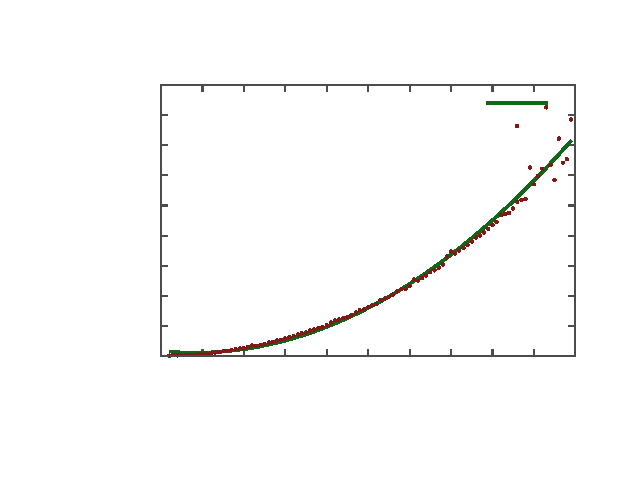
\includegraphics{./graficos/ajuste-clasico-v2}}%
    \gplfronttext
  \end{picture}%
\endgroup

	}
	\end{center}
\end{frame}

\begin{frame}{Divide y Vencerás}

	Hemos realizado dos algoritmos usando la técnica Divide y Vencerás:
	\begin{itemize}
		\item Vectores dinámicos
		\item Vectores de la STL
	\end{itemize}
\end{frame}

\begin{frame}{Vectores Dinámicos}

	\lstinputlisting[language=C++, linerange={83-104}]{./src/mezcla-vectores-DyV.cpp}
\end{frame}

\begin{frame}{Eficiencia teórica}
    \vspace{-1em}
    Consideramos que $n$ es una constante fija.
    
    \vskip 1cm 
	Ecuación general: $$ \begin{cases} T(1) = 1\\ T(k) = 2T\left(\frac{k}{2}\right) + n\frac{k}{2} \end{cases} $$
	Orden de eficiencia: $$ O\left(\frac{n}{2}k\log k \right) \thicksim O(k\log k) $$
\end{frame}


\begin{frame}{Eficiencia empírica}

	\begin{center}
	\resizebox*{11cm}{!}{
		% GNUPLOT: LaTeX picture with Postscript
\begingroup
  \makeatletter
  \providecommand\color[2][]{%
    \GenericError{(gnuplot) \space\space\space\@spaces}{%
      Package color not loaded in conjunction with
      terminal option `colourtext'%
    }{See the gnuplot documentation for explanation.%
    }{Either use 'blacktext' in gnuplot or load the package
      color.sty in LaTeX.}%
    \renewcommand\color[2][]{}%
  }%
  \providecommand\includegraphics[2][]{%
    \GenericError{(gnuplot) \space\space\space\@spaces}{%
      Package graphicx or graphics not loaded%
    }{See the gnuplot documentation for explanation.%
    }{The gnuplot epslatex terminal needs graphicx.sty or graphics.sty.}%
    \renewcommand\includegraphics[2][]{}%
  }%
  \providecommand\rotatebox[2]{#2}%
  \@ifundefined{ifGPcolor}{%
    \newif\ifGPcolor
    \GPcolortrue
  }{}%
  \@ifundefined{ifGPblacktext}{%
    \newif\ifGPblacktext
    \GPblacktextfalse
  }{}%
  % define a \g@addto@macro without @ in the name:
  \let\gplgaddtomacro\g@addto@macro
  % define empty templates for all commands taking text:
  \gdef\gplbacktext{}%
  \gdef\gplfronttext{}%
  \makeatother
  \ifGPblacktext
    % no textcolor at all
    \def\colorrgb#1{}%
    \def\colorgray#1{}%
  \else
    % gray or color?
    \ifGPcolor
      \def\colorrgb#1{\color[rgb]{#1}}%
      \def\colorgray#1{\color[gray]{#1}}%
      \expandafter\def\csname LTw\endcsname{\color{white}}%
      \expandafter\def\csname LTb\endcsname{\color{black}}%
      \expandafter\def\csname LTa\endcsname{\color{black}}%
      \expandafter\def\csname LT0\endcsname{\color[rgb]{1,0,0}}%
      \expandafter\def\csname LT1\endcsname{\color[rgb]{0,1,0}}%
      \expandafter\def\csname LT2\endcsname{\color[rgb]{0,0,1}}%
      \expandafter\def\csname LT3\endcsname{\color[rgb]{1,0,1}}%
      \expandafter\def\csname LT4\endcsname{\color[rgb]{0,1,1}}%
      \expandafter\def\csname LT5\endcsname{\color[rgb]{1,1,0}}%
      \expandafter\def\csname LT6\endcsname{\color[rgb]{0,0,0}}%
      \expandafter\def\csname LT7\endcsname{\color[rgb]{1,0.3,0}}%
      \expandafter\def\csname LT8\endcsname{\color[rgb]{0.5,0.5,0.5}}%
    \else
      % gray
      \def\colorrgb#1{\color{black}}%
      \def\colorgray#1{\color[gray]{#1}}%
      \expandafter\def\csname LTw\endcsname{\color{white}}%
      \expandafter\def\csname LTb\endcsname{\color{black}}%
      \expandafter\def\csname LTa\endcsname{\color{black}}%
      \expandafter\def\csname LT0\endcsname{\color{black}}%
      \expandafter\def\csname LT1\endcsname{\color{black}}%
      \expandafter\def\csname LT2\endcsname{\color{black}}%
      \expandafter\def\csname LT3\endcsname{\color{black}}%
      \expandafter\def\csname LT4\endcsname{\color{black}}%
      \expandafter\def\csname LT5\endcsname{\color{black}}%
      \expandafter\def\csname LT6\endcsname{\color{black}}%
      \expandafter\def\csname LT7\endcsname{\color{black}}%
      \expandafter\def\csname LT8\endcsname{\color{black}}%
    \fi
  \fi
    \setlength{\unitlength}{0.0500bp}%
    \ifx\gptboxheight\undefined%
      \newlength{\gptboxheight}%
      \newlength{\gptboxwidth}%
      \newsavebox{\gptboxtext}%
    \fi%
    \setlength{\fboxrule}{0.5pt}%
    \setlength{\fboxsep}{1pt}%
\begin{picture}(7200.00,4320.00)%
    \gplgaddtomacro\gplbacktext{%
      \colorrgb{0.30,0.30,0.30}%
      \put(1518,1060){\makebox(0,0)[r]{\strut{}$\textcolor{text}{0}$}}%
      \colorrgb{0.30,0.30,0.30}%
      \put(1518,1431){\makebox(0,0)[r]{\strut{}$\textcolor{text}{0.001}$}}%
      \colorrgb{0.30,0.30,0.30}%
      \put(1518,1803){\makebox(0,0)[r]{\strut{}$\textcolor{text}{0.002}$}}%
      \colorrgb{0.30,0.30,0.30}%
      \put(1518,2174){\makebox(0,0)[r]{\strut{}$\textcolor{text}{0.003}$}}%
      \colorrgb{0.30,0.30,0.30}%
      \put(1518,2545){\makebox(0,0)[r]{\strut{}$\textcolor{text}{0.004}$}}%
      \colorrgb{0.30,0.30,0.30}%
      \put(1518,2916){\makebox(0,0)[r]{\strut{}$\textcolor{text}{0.005}$}}%
      \colorrgb{0.30,0.30,0.30}%
      \put(1518,3288){\makebox(0,0)[r]{\strut{}$\textcolor{text}{0.006}$}}%
      \colorrgb{0.30,0.30,0.30}%
      \put(1518,3659){\makebox(0,0)[r]{\strut{}$\textcolor{text}{0.007}$}}%
      \colorrgb{0.30,0.30,0.30}%
      \put(1650,928){\rotatebox{45}{\makebox(0,0)[r]{\strut{}$\textcolor{text}{0}$}}}%
      \colorrgb{0.30,0.30,0.30}%
      \put(2165,928){\rotatebox{45}{\makebox(0,0)[r]{\strut{}$\textcolor{text}{500}$}}}%
      \colorrgb{0.30,0.30,0.30}%
      \put(2681,928){\rotatebox{45}{\makebox(0,0)[r]{\strut{}$\textcolor{text}{1000}$}}}%
      \colorrgb{0.30,0.30,0.30}%
      \put(3196,928){\rotatebox{45}{\makebox(0,0)[r]{\strut{}$\textcolor{text}{1500}$}}}%
      \colorrgb{0.30,0.30,0.30}%
      \put(3711,928){\rotatebox{45}{\makebox(0,0)[r]{\strut{}$\textcolor{text}{2000}$}}}%
      \colorrgb{0.30,0.30,0.30}%
      \put(4227,928){\rotatebox{45}{\makebox(0,0)[r]{\strut{}$\textcolor{text}{2500}$}}}%
      \colorrgb{0.30,0.30,0.30}%
      \put(4742,928){\rotatebox{45}{\makebox(0,0)[r]{\strut{}$\textcolor{text}{3000}$}}}%
      \colorrgb{0.30,0.30,0.30}%
      \put(5257,928){\rotatebox{45}{\makebox(0,0)[r]{\strut{}$\textcolor{text}{3500}$}}}%
      \colorrgb{0.30,0.30,0.30}%
      \put(5772,928){\rotatebox{45}{\makebox(0,0)[r]{\strut{}$\textcolor{text}{4000}$}}}%
      \colorrgb{0.30,0.30,0.30}%
      \put(6288,928){\rotatebox{45}{\makebox(0,0)[r]{\strut{}$\textcolor{text}{4500}$}}}%
      \colorrgb{0.30,0.30,0.30}%
      \put(6803,928){\rotatebox{45}{\makebox(0,0)[r]{\strut{}$\textcolor{text}{5000}$}}}%
    }%
    \gplgaddtomacro\gplfronttext{%
      \colorrgb{0.30,0.30,0.30}%
      \put(220,2359){\rotatebox{-270}{\makebox(0,0){\strut{}Tiempo de ejecución (s)}}}%
      \colorrgb{0.30,0.30,0.30}%
      \put(4226,220){\makebox(0,0){\strut{}Número de vectores (k)}}%
      \colorrgb{0.30,0.30,0.30}%
      \put(4226,3989){\makebox(0,0){\strut{}Eficiencia empírica mezcla-vectores-DyV}}%
      \csname LTb\endcsname%
      \put(5816,3486){\makebox(0,0)[r]{\strut{}Algoritmo divide y vencerás n = 10}}%
    }%
    \gplbacktext
    \put(0,0){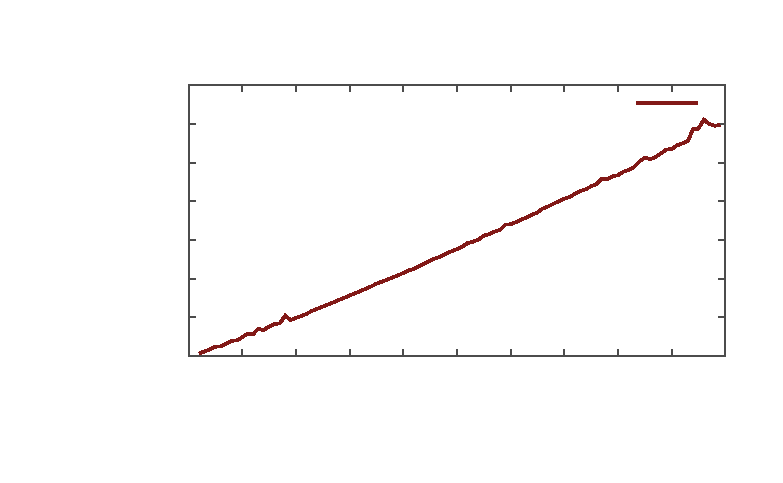
\includegraphics{graficos/mezcla-vectores-DyV}}%
    \gplfronttext
  \end{picture}%
\endgroup

	}
	\end{center}
\end{frame}

\begin{frame}{Eficiencia híbrida}

	\begin{center}
	\resizebox*{10cm}{!}{
		% GNUPLOT: LaTeX picture with Postscript
\begingroup
  \makeatletter
  \providecommand\color[2][]{%
    \GenericError{(gnuplot) \space\space\space\@spaces}{%
      Package color not loaded in conjunction with
      terminal option `colourtext'%
    }{See the gnuplot documentation for explanation.%
    }{Either use 'blacktext' in gnuplot or load the package
      color.sty in LaTeX.}%
    \renewcommand\color[2][]{}%
  }%
  \providecommand\includegraphics[2][]{%
    \GenericError{(gnuplot) \space\space\space\@spaces}{%
      Package graphicx or graphics not loaded%
    }{See the gnuplot documentation for explanation.%
    }{The gnuplot epslatex terminal needs graphicx.sty or graphics.sty.}%
    \renewcommand\includegraphics[2][]{}%
  }%
  \providecommand\rotatebox[2]{#2}%
  \@ifundefined{ifGPcolor}{%
    \newif\ifGPcolor
    \GPcolortrue
  }{}%
  \@ifundefined{ifGPblacktext}{%
    \newif\ifGPblacktext
    \GPblacktextfalse
  }{}%
  % define a \g@addto@macro without @ in the name:
  \let\gplgaddtomacro\g@addto@macro
  % define empty templates for all commands taking text:
  \gdef\gplbacktext{}%
  \gdef\gplfronttext{}%
  \makeatother
  \ifGPblacktext
    % no textcolor at all
    \def\colorrgb#1{}%
    \def\colorgray#1{}%
  \else
    % gray or color?
    \ifGPcolor
      \def\colorrgb#1{\color[rgb]{#1}}%
      \def\colorgray#1{\color[gray]{#1}}%
      \expandafter\def\csname LTw\endcsname{\color{white}}%
      \expandafter\def\csname LTb\endcsname{\color{black}}%
      \expandafter\def\csname LTa\endcsname{\color{black}}%
      \expandafter\def\csname LT0\endcsname{\color[rgb]{1,0,0}}%
      \expandafter\def\csname LT1\endcsname{\color[rgb]{0,1,0}}%
      \expandafter\def\csname LT2\endcsname{\color[rgb]{0,0,1}}%
      \expandafter\def\csname LT3\endcsname{\color[rgb]{1,0,1}}%
      \expandafter\def\csname LT4\endcsname{\color[rgb]{0,1,1}}%
      \expandafter\def\csname LT5\endcsname{\color[rgb]{1,1,0}}%
      \expandafter\def\csname LT6\endcsname{\color[rgb]{0,0,0}}%
      \expandafter\def\csname LT7\endcsname{\color[rgb]{1,0.3,0}}%
      \expandafter\def\csname LT8\endcsname{\color[rgb]{0.5,0.5,0.5}}%
    \else
      % gray
      \def\colorrgb#1{\color{black}}%
      \def\colorgray#1{\color[gray]{#1}}%
      \expandafter\def\csname LTw\endcsname{\color{white}}%
      \expandafter\def\csname LTb\endcsname{\color{black}}%
      \expandafter\def\csname LTa\endcsname{\color{black}}%
      \expandafter\def\csname LT0\endcsname{\color{black}}%
      \expandafter\def\csname LT1\endcsname{\color{black}}%
      \expandafter\def\csname LT2\endcsname{\color{black}}%
      \expandafter\def\csname LT3\endcsname{\color{black}}%
      \expandafter\def\csname LT4\endcsname{\color{black}}%
      \expandafter\def\csname LT5\endcsname{\color{black}}%
      \expandafter\def\csname LT6\endcsname{\color{black}}%
      \expandafter\def\csname LT7\endcsname{\color{black}}%
      \expandafter\def\csname LT8\endcsname{\color{black}}%
    \fi
  \fi
    \setlength{\unitlength}{0.0500bp}%
    \ifx\gptboxheight\undefined%
      \newlength{\gptboxheight}%
      \newlength{\gptboxwidth}%
      \newsavebox{\gptboxtext}%
    \fi%
    \setlength{\fboxrule}{0.5pt}%
    \setlength{\fboxsep}{1pt}%
\begin{picture}(5760.00,4320.00)%
    \gplgaddtomacro\gplbacktext{%
      \colorrgb{0.30,0.30,0.30}%
      \put(1518,1060){\makebox(0,0)[r]{\strut{}$\textcolor{text}{0}$}}%
      \colorrgb{0.30,0.30,0.30}%
      \put(1518,1431){\makebox(0,0)[r]{\strut{}$\textcolor{text}{0.001}$}}%
      \colorrgb{0.30,0.30,0.30}%
      \put(1518,1803){\makebox(0,0)[r]{\strut{}$\textcolor{text}{0.002}$}}%
      \colorrgb{0.30,0.30,0.30}%
      \put(1518,2174){\makebox(0,0)[r]{\strut{}$\textcolor{text}{0.003}$}}%
      \colorrgb{0.30,0.30,0.30}%
      \put(1518,2545){\makebox(0,0)[r]{\strut{}$\textcolor{text}{0.004}$}}%
      \colorrgb{0.30,0.30,0.30}%
      \put(1518,2916){\makebox(0,0)[r]{\strut{}$\textcolor{text}{0.005}$}}%
      \colorrgb{0.30,0.30,0.30}%
      \put(1518,3288){\makebox(0,0)[r]{\strut{}$\textcolor{text}{0.006}$}}%
      \colorrgb{0.30,0.30,0.30}%
      \put(1518,3659){\makebox(0,0)[r]{\strut{}$\textcolor{text}{0.007}$}}%
      \colorrgb{0.30,0.30,0.30}%
      \put(1650,928){\rotatebox{45}{\makebox(0,0)[r]{\strut{}$\textcolor{text}{0}$}}}%
      \colorrgb{0.30,0.30,0.30}%
      \put(2021,928){\rotatebox{45}{\makebox(0,0)[r]{\strut{}$\textcolor{text}{500}$}}}%
      \colorrgb{0.30,0.30,0.30}%
      \put(2393,928){\rotatebox{45}{\makebox(0,0)[r]{\strut{}$\textcolor{text}{1000}$}}}%
      \colorrgb{0.30,0.30,0.30}%
      \put(2764,928){\rotatebox{45}{\makebox(0,0)[r]{\strut{}$\textcolor{text}{1500}$}}}%
      \colorrgb{0.30,0.30,0.30}%
      \put(3135,928){\rotatebox{45}{\makebox(0,0)[r]{\strut{}$\textcolor{text}{2000}$}}}%
      \colorrgb{0.30,0.30,0.30}%
      \put(3507,928){\rotatebox{45}{\makebox(0,0)[r]{\strut{}$\textcolor{text}{2500}$}}}%
      \colorrgb{0.30,0.30,0.30}%
      \put(3878,928){\rotatebox{45}{\makebox(0,0)[r]{\strut{}$\textcolor{text}{3000}$}}}%
      \colorrgb{0.30,0.30,0.30}%
      \put(4249,928){\rotatebox{45}{\makebox(0,0)[r]{\strut{}$\textcolor{text}{3500}$}}}%
      \colorrgb{0.30,0.30,0.30}%
      \put(4620,928){\rotatebox{45}{\makebox(0,0)[r]{\strut{}$\textcolor{text}{4000}$}}}%
      \colorrgb{0.30,0.30,0.30}%
      \put(4992,928){\rotatebox{45}{\makebox(0,0)[r]{\strut{}$\textcolor{text}{4500}$}}}%
      \colorrgb{0.30,0.30,0.30}%
      \put(5363,928){\rotatebox{45}{\makebox(0,0)[r]{\strut{}$\textcolor{text}{5000}$}}}%
    }%
    \gplgaddtomacro\gplfronttext{%
      \colorrgb{0.30,0.30,0.30}%
      \put(220,2359){\rotatebox{-270}{\makebox(0,0){\strut{}Tiempo de ejecución (s)}}}%
      \colorrgb{0.30,0.30,0.30}%
      \put(3506,220){\makebox(0,0){\strut{}Tamaño del vector (elementos)}}%
      \colorrgb{0.30,0.30,0.30}%
      \put(3506,3989){\makebox(0,0){\strut{}Ajuste algoritmo divide y vencerás}}%
      \csname LTb\endcsname%
      \put(4376,3486){\makebox(0,0)[r]{\strut{}$ 1.42e-08 \cdot k\log k + 7.20e-06 k + %2.2e$}}%
      \csname LTb\endcsname%
      \put(4376,3266){\makebox(0,0)[r]{\strut{}Divide y vencerás}}%
    }%
    \gplbacktext
    \put(0,0){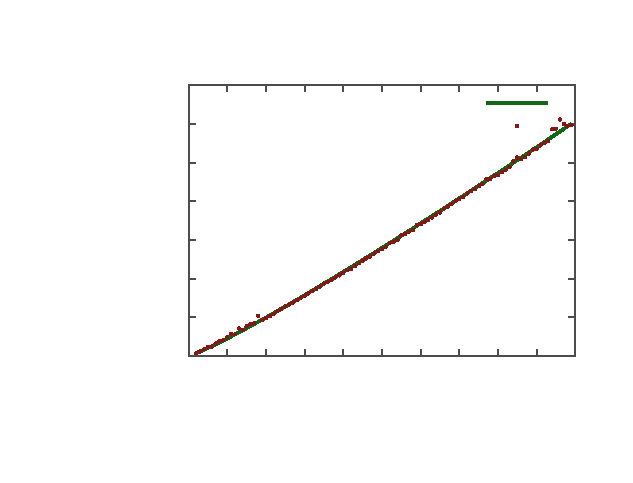
\includegraphics{./graficos/ajuste-DyV}}%
    \gplfronttext
  \end{picture}%
\endgroup

	}
	\end{center}
\end{frame}

\begin{frame}{Vectores de la STL}

	\lstinputlisting[language=C++, linerange={75-96}]{./src/mezcla-vectores-DyV-STL.cpp}
\end{frame}

\begin{frame}{Eficiencia empírica}

	\begin{center}
	\resizebox*{11cm}{!}{
		% GNUPLOT: LaTeX picture with Postscript
\begingroup
  \makeatletter
  \providecommand\color[2][]{%
    \GenericError{(gnuplot) \space\space\space\@spaces}{%
      Package color not loaded in conjunction with
      terminal option `colourtext'%
    }{See the gnuplot documentation for explanation.%
    }{Either use 'blacktext' in gnuplot or load the package
      color.sty in LaTeX.}%
    \renewcommand\color[2][]{}%
  }%
  \providecommand\includegraphics[2][]{%
    \GenericError{(gnuplot) \space\space\space\@spaces}{%
      Package graphicx or graphics not loaded%
    }{See the gnuplot documentation for explanation.%
    }{The gnuplot epslatex terminal needs graphicx.sty or graphics.sty.}%
    \renewcommand\includegraphics[2][]{}%
  }%
  \providecommand\rotatebox[2]{#2}%
  \@ifundefined{ifGPcolor}{%
    \newif\ifGPcolor
    \GPcolortrue
  }{}%
  \@ifundefined{ifGPblacktext}{%
    \newif\ifGPblacktext
    \GPblacktextfalse
  }{}%
  % define a \g@addto@macro without @ in the name:
  \let\gplgaddtomacro\g@addto@macro
  % define empty templates for all commands taking text:
  \gdef\gplbacktext{}%
  \gdef\gplfronttext{}%
  \makeatother
  \ifGPblacktext
    % no textcolor at all
    \def\colorrgb#1{}%
    \def\colorgray#1{}%
  \else
    % gray or color?
    \ifGPcolor
      \def\colorrgb#1{\color[rgb]{#1}}%
      \def\colorgray#1{\color[gray]{#1}}%
      \expandafter\def\csname LTw\endcsname{\color{white}}%
      \expandafter\def\csname LTb\endcsname{\color{black}}%
      \expandafter\def\csname LTa\endcsname{\color{black}}%
      \expandafter\def\csname LT0\endcsname{\color[rgb]{1,0,0}}%
      \expandafter\def\csname LT1\endcsname{\color[rgb]{0,1,0}}%
      \expandafter\def\csname LT2\endcsname{\color[rgb]{0,0,1}}%
      \expandafter\def\csname LT3\endcsname{\color[rgb]{1,0,1}}%
      \expandafter\def\csname LT4\endcsname{\color[rgb]{0,1,1}}%
      \expandafter\def\csname LT5\endcsname{\color[rgb]{1,1,0}}%
      \expandafter\def\csname LT6\endcsname{\color[rgb]{0,0,0}}%
      \expandafter\def\csname LT7\endcsname{\color[rgb]{1,0.3,0}}%
      \expandafter\def\csname LT8\endcsname{\color[rgb]{0.5,0.5,0.5}}%
    \else
      % gray
      \def\colorrgb#1{\color{black}}%
      \def\colorgray#1{\color[gray]{#1}}%
      \expandafter\def\csname LTw\endcsname{\color{white}}%
      \expandafter\def\csname LTb\endcsname{\color{black}}%
      \expandafter\def\csname LTa\endcsname{\color{black}}%
      \expandafter\def\csname LT0\endcsname{\color{black}}%
      \expandafter\def\csname LT1\endcsname{\color{black}}%
      \expandafter\def\csname LT2\endcsname{\color{black}}%
      \expandafter\def\csname LT3\endcsname{\color{black}}%
      \expandafter\def\csname LT4\endcsname{\color{black}}%
      \expandafter\def\csname LT5\endcsname{\color{black}}%
      \expandafter\def\csname LT6\endcsname{\color{black}}%
      \expandafter\def\csname LT7\endcsname{\color{black}}%
      \expandafter\def\csname LT8\endcsname{\color{black}}%
    \fi
  \fi
    \setlength{\unitlength}{0.0500bp}%
    \ifx\gptboxheight\undefined%
      \newlength{\gptboxheight}%
      \newlength{\gptboxwidth}%
      \newsavebox{\gptboxtext}%
    \fi%
    \setlength{\fboxrule}{0.5pt}%
    \setlength{\fboxsep}{1pt}%
\begin{picture}(7200.00,4320.00)%
    \gplgaddtomacro\gplbacktext{%
      \colorrgb{0.30,0.30,0.30}%
      \put(1518,1060){\makebox(0,0)[r]{\strut{}$\textcolor{text}{0}$}}%
      \colorrgb{0.30,0.30,0.30}%
      \put(1518,1431){\makebox(0,0)[r]{\strut{}$\textcolor{text}{0.005}$}}%
      \colorrgb{0.30,0.30,0.30}%
      \put(1518,1803){\makebox(0,0)[r]{\strut{}$\textcolor{text}{0.01}$}}%
      \colorrgb{0.30,0.30,0.30}%
      \put(1518,2174){\makebox(0,0)[r]{\strut{}$\textcolor{text}{0.015}$}}%
      \colorrgb{0.30,0.30,0.30}%
      \put(1518,2545){\makebox(0,0)[r]{\strut{}$\textcolor{text}{0.02}$}}%
      \colorrgb{0.30,0.30,0.30}%
      \put(1518,2916){\makebox(0,0)[r]{\strut{}$\textcolor{text}{0.025}$}}%
      \colorrgb{0.30,0.30,0.30}%
      \put(1518,3288){\makebox(0,0)[r]{\strut{}$\textcolor{text}{0.03}$}}%
      \colorrgb{0.30,0.30,0.30}%
      \put(1518,3659){\makebox(0,0)[r]{\strut{}$\textcolor{text}{0.035}$}}%
      \colorrgb{0.30,0.30,0.30}%
      \put(1650,928){\rotatebox{45}{\makebox(0,0)[r]{\strut{}$\textcolor{text}{0}$}}}%
      \colorrgb{0.30,0.30,0.30}%
      \put(2165,928){\rotatebox{45}{\makebox(0,0)[r]{\strut{}$\textcolor{text}{500}$}}}%
      \colorrgb{0.30,0.30,0.30}%
      \put(2681,928){\rotatebox{45}{\makebox(0,0)[r]{\strut{}$\textcolor{text}{1000}$}}}%
      \colorrgb{0.30,0.30,0.30}%
      \put(3196,928){\rotatebox{45}{\makebox(0,0)[r]{\strut{}$\textcolor{text}{1500}$}}}%
      \colorrgb{0.30,0.30,0.30}%
      \put(3711,928){\rotatebox{45}{\makebox(0,0)[r]{\strut{}$\textcolor{text}{2000}$}}}%
      \colorrgb{0.30,0.30,0.30}%
      \put(4227,928){\rotatebox{45}{\makebox(0,0)[r]{\strut{}$\textcolor{text}{2500}$}}}%
      \colorrgb{0.30,0.30,0.30}%
      \put(4742,928){\rotatebox{45}{\makebox(0,0)[r]{\strut{}$\textcolor{text}{3000}$}}}%
      \colorrgb{0.30,0.30,0.30}%
      \put(5257,928){\rotatebox{45}{\makebox(0,0)[r]{\strut{}$\textcolor{text}{3500}$}}}%
      \colorrgb{0.30,0.30,0.30}%
      \put(5772,928){\rotatebox{45}{\makebox(0,0)[r]{\strut{}$\textcolor{text}{4000}$}}}%
      \colorrgb{0.30,0.30,0.30}%
      \put(6288,928){\rotatebox{45}{\makebox(0,0)[r]{\strut{}$\textcolor{text}{4500}$}}}%
      \colorrgb{0.30,0.30,0.30}%
      \put(6803,928){\rotatebox{45}{\makebox(0,0)[r]{\strut{}$\textcolor{text}{5000}$}}}%
    }%
    \gplgaddtomacro\gplfronttext{%
      \colorrgb{0.30,0.30,0.30}%
      \put(220,2359){\rotatebox{-270}{\makebox(0,0){\strut{}Tiempo de ejecución (s)}}}%
      \colorrgb{0.30,0.30,0.30}%
      \put(4226,220){\makebox(0,0){\strut{}Número de vectores (k)}}%
      \colorrgb{0.30,0.30,0.30}%
      \put(4226,3989){\makebox(0,0){\strut{}Eficiencia empírica mezcla-vectores-DyV-STL}}%
      \csname LTb\endcsname%
      \put(5816,3486){\makebox(0,0)[r]{\strut{}Algoritmo divide y vencerás n = 10}}%
    }%
    \gplbacktext
    \put(0,0){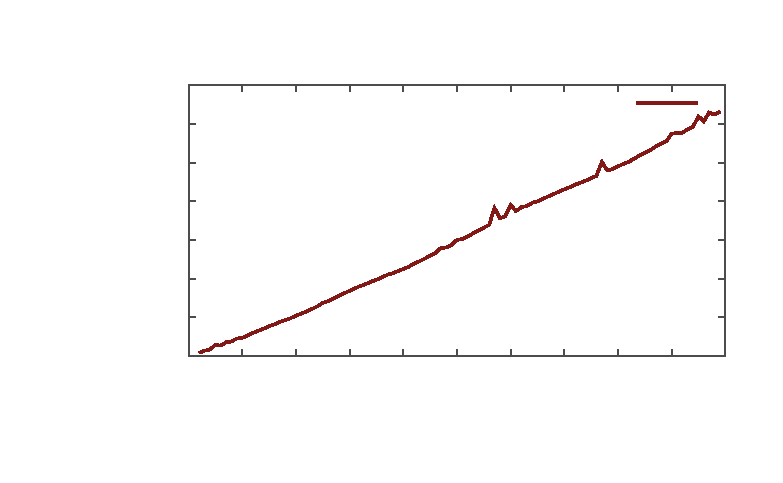
\includegraphics{graficos/mezcla-vectores-DyV-STL}}%
    \gplfronttext
  \end{picture}%
\endgroup

	}
	\end{center}
\end{frame}

\begin{frame}{Eficiencia híbrida}
  \fontsize{8pt}{7.2}\selectfont
	\begin{center}
	\resizebox*{10cm}{!}{
		% GNUPLOT: LaTeX picture with Postscript
\begingroup
  \makeatletter
  \providecommand\color[2][]{%
    \GenericError{(gnuplot) \space\space\space\@spaces}{%
      Package color not loaded in conjunction with
      terminal option `colourtext'%
    }{See the gnuplot documentation for explanation.%
    }{Either use 'blacktext' in gnuplot or load the package
      color.sty in LaTeX.}%
    \renewcommand\color[2][]{}%
  }%
  \providecommand\includegraphics[2][]{%
    \GenericError{(gnuplot) \space\space\space\@spaces}{%
      Package graphicx or graphics not loaded%
    }{See the gnuplot documentation for explanation.%
    }{The gnuplot epslatex terminal needs graphicx.sty or graphics.sty.}%
    \renewcommand\includegraphics[2][]{}%
  }%
  \providecommand\rotatebox[2]{#2}%
  \@ifundefined{ifGPcolor}{%
    \newif\ifGPcolor
    \GPcolortrue
  }{}%
  \@ifundefined{ifGPblacktext}{%
    \newif\ifGPblacktext
    \GPblacktextfalse
  }{}%
  % define a \g@addto@macro without @ in the name:
  \let\gplgaddtomacro\g@addto@macro
  % define empty templates for all commands taking text:
  \gdef\gplbacktext{}%
  \gdef\gplfronttext{}%
  \makeatother
  \ifGPblacktext
    % no textcolor at all
    \def\colorrgb#1{}%
    \def\colorgray#1{}%
  \else
    % gray or color?
    \ifGPcolor
      \def\colorrgb#1{\color[rgb]{#1}}%
      \def\colorgray#1{\color[gray]{#1}}%
      \expandafter\def\csname LTw\endcsname{\color{white}}%
      \expandafter\def\csname LTb\endcsname{\color{black}}%
      \expandafter\def\csname LTa\endcsname{\color{black}}%
      \expandafter\def\csname LT0\endcsname{\color[rgb]{1,0,0}}%
      \expandafter\def\csname LT1\endcsname{\color[rgb]{0,1,0}}%
      \expandafter\def\csname LT2\endcsname{\color[rgb]{0,0,1}}%
      \expandafter\def\csname LT3\endcsname{\color[rgb]{1,0,1}}%
      \expandafter\def\csname LT4\endcsname{\color[rgb]{0,1,1}}%
      \expandafter\def\csname LT5\endcsname{\color[rgb]{1,1,0}}%
      \expandafter\def\csname LT6\endcsname{\color[rgb]{0,0,0}}%
      \expandafter\def\csname LT7\endcsname{\color[rgb]{1,0.3,0}}%
      \expandafter\def\csname LT8\endcsname{\color[rgb]{0.5,0.5,0.5}}%
    \else
      % gray
      \def\colorrgb#1{\color{black}}%
      \def\colorgray#1{\color[gray]{#1}}%
      \expandafter\def\csname LTw\endcsname{\color{white}}%
      \expandafter\def\csname LTb\endcsname{\color{black}}%
      \expandafter\def\csname LTa\endcsname{\color{black}}%
      \expandafter\def\csname LT0\endcsname{\color{black}}%
      \expandafter\def\csname LT1\endcsname{\color{black}}%
      \expandafter\def\csname LT2\endcsname{\color{black}}%
      \expandafter\def\csname LT3\endcsname{\color{black}}%
      \expandafter\def\csname LT4\endcsname{\color{black}}%
      \expandafter\def\csname LT5\endcsname{\color{black}}%
      \expandafter\def\csname LT6\endcsname{\color{black}}%
      \expandafter\def\csname LT7\endcsname{\color{black}}%
      \expandafter\def\csname LT8\endcsname{\color{black}}%
    \fi
  \fi
    \setlength{\unitlength}{0.0500bp}%
    \ifx\gptboxheight\undefined%
      \newlength{\gptboxheight}%
      \newlength{\gptboxwidth}%
      \newsavebox{\gptboxtext}%
    \fi%
    \setlength{\fboxrule}{0.5pt}%
    \setlength{\fboxsep}{1pt}%
\begin{picture}(5760.00,4320.00)%
    \gplgaddtomacro\gplbacktext{%
      \colorrgb{0.30,0.30,0.30}%
      \put(1518,1060){\makebox(0,0)[r]{\strut{}$\textcolor{text}{0}$}}%
      \colorrgb{0.30,0.30,0.30}%
      \put(1518,1431){\makebox(0,0)[r]{\strut{}$\textcolor{text}{0.005}$}}%
      \colorrgb{0.30,0.30,0.30}%
      \put(1518,1803){\makebox(0,0)[r]{\strut{}$\textcolor{text}{0.01}$}}%
      \colorrgb{0.30,0.30,0.30}%
      \put(1518,2174){\makebox(0,0)[r]{\strut{}$\textcolor{text}{0.015}$}}%
      \colorrgb{0.30,0.30,0.30}%
      \put(1518,2545){\makebox(0,0)[r]{\strut{}$\textcolor{text}{0.02}$}}%
      \colorrgb{0.30,0.30,0.30}%
      \put(1518,2916){\makebox(0,0)[r]{\strut{}$\textcolor{text}{0.025}$}}%
      \colorrgb{0.30,0.30,0.30}%
      \put(1518,3288){\makebox(0,0)[r]{\strut{}$\textcolor{text}{0.03}$}}%
      \colorrgb{0.30,0.30,0.30}%
      \put(1518,3659){\makebox(0,0)[r]{\strut{}$\textcolor{text}{0.035}$}}%
      \colorrgb{0.30,0.30,0.30}%
      \put(1650,928){\rotatebox{45}{\makebox(0,0)[r]{\strut{}$\textcolor{text}{0}$}}}%
      \colorrgb{0.30,0.30,0.30}%
      \put(2021,928){\rotatebox{45}{\makebox(0,0)[r]{\strut{}$\textcolor{text}{500}$}}}%
      \colorrgb{0.30,0.30,0.30}%
      \put(2393,928){\rotatebox{45}{\makebox(0,0)[r]{\strut{}$\textcolor{text}{1000}$}}}%
      \colorrgb{0.30,0.30,0.30}%
      \put(2764,928){\rotatebox{45}{\makebox(0,0)[r]{\strut{}$\textcolor{text}{1500}$}}}%
      \colorrgb{0.30,0.30,0.30}%
      \put(3135,928){\rotatebox{45}{\makebox(0,0)[r]{\strut{}$\textcolor{text}{2000}$}}}%
      \colorrgb{0.30,0.30,0.30}%
      \put(3507,928){\rotatebox{45}{\makebox(0,0)[r]{\strut{}$\textcolor{text}{2500}$}}}%
      \colorrgb{0.30,0.30,0.30}%
      \put(3878,928){\rotatebox{45}{\makebox(0,0)[r]{\strut{}$\textcolor{text}{3000}$}}}%
      \colorrgb{0.30,0.30,0.30}%
      \put(4249,928){\rotatebox{45}{\makebox(0,0)[r]{\strut{}$\textcolor{text}{3500}$}}}%
      \colorrgb{0.30,0.30,0.30}%
      \put(4620,928){\rotatebox{45}{\makebox(0,0)[r]{\strut{}$\textcolor{text}{4000}$}}}%
      \colorrgb{0.30,0.30,0.30}%
      \put(4992,928){\rotatebox{45}{\makebox(0,0)[r]{\strut{}$\textcolor{text}{4500}$}}}%
      \colorrgb{0.30,0.30,0.30}%
      \put(5363,928){\rotatebox{45}{\makebox(0,0)[r]{\strut{}$\textcolor{text}{5000}$}}}%
    }%
    \gplgaddtomacro\gplfronttext{%
      \colorrgb{0.30,0.30,0.30}%
      \put(220,2359){\rotatebox{-270}{\makebox(0,0){\strut{}Tiempo de ejecución (s)}}}%
      \colorrgb{0.30,0.30,0.30}%
      \put(3506,220){\makebox(0,0){\strut{}Tamaño del vector (elementos)}}%
      \colorrgb{0.30,0.30,0.30}%
      \put(3506,3989){\makebox(0,0){\strut{}Ajuste algoritmo divide y vencerás STL}}%
      \csname LTb\endcsname%
      \put(4376,3486){\makebox(0,0)[r]{\strut{}7.49e-08 $ \cdot klog k +$ 1.33e-04}}%
      \csname LTb\endcsname%
      \put(4376,3266){\makebox(0,0)[r]{\strut{}Divide y vencerás STL}}%
    }%
    \gplbacktext
    \put(0,0){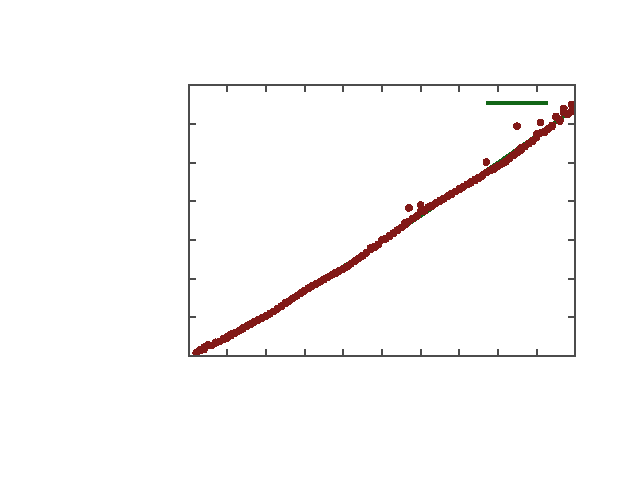
\includegraphics{./graficos/ajuste-DyV-STL}}%
    \gplfronttext
  \end{picture}%
\endgroup

	}
	\end{center}

\end{frame}

\begin{frame}{Comparación eficiencias}
	
	\begin{center}
	\resizebox*{11cm}{!}{
		% GNUPLOT: LaTeX picture with Postscript
\begingroup
  \makeatletter
  \providecommand\color[2][]{%
    \GenericError{(gnuplot) \space\space\space\@spaces}{%
      Package color not loaded in conjunction with
      terminal option `colourtext'%
    }{See the gnuplot documentation for explanation.%
    }{Either use 'blacktext' in gnuplot or load the package
      color.sty in LaTeX.}%
    \renewcommand\color[2][]{}%
  }%
  \providecommand\includegraphics[2][]{%
    \GenericError{(gnuplot) \space\space\space\@spaces}{%
      Package graphicx or graphics not loaded%
    }{See the gnuplot documentation for explanation.%
    }{The gnuplot epslatex terminal needs graphicx.sty or graphics.sty.}%
    \renewcommand\includegraphics[2][]{}%
  }%
  \providecommand\rotatebox[2]{#2}%
  \@ifundefined{ifGPcolor}{%
    \newif\ifGPcolor
    \GPcolortrue
  }{}%
  \@ifundefined{ifGPblacktext}{%
    \newif\ifGPblacktext
    \GPblacktextfalse
  }{}%
  % define a \g@addto@macro without @ in the name:
  \let\gplgaddtomacro\g@addto@macro
  % define empty templates for all commands taking text:
  \gdef\gplbacktext{}%
  \gdef\gplfronttext{}%
  \makeatother
  \ifGPblacktext
    % no textcolor at all
    \def\colorrgb#1{}%
    \def\colorgray#1{}%
  \else
    % gray or color?
    \ifGPcolor
      \def\colorrgb#1{\color[rgb]{#1}}%
      \def\colorgray#1{\color[gray]{#1}}%
      \expandafter\def\csname LTw\endcsname{\color{white}}%
      \expandafter\def\csname LTb\endcsname{\color{black}}%
      \expandafter\def\csname LTa\endcsname{\color{black}}%
      \expandafter\def\csname LT0\endcsname{\color[rgb]{1,0,0}}%
      \expandafter\def\csname LT1\endcsname{\color[rgb]{0,1,0}}%
      \expandafter\def\csname LT2\endcsname{\color[rgb]{0,0,1}}%
      \expandafter\def\csname LT3\endcsname{\color[rgb]{1,0,1}}%
      \expandafter\def\csname LT4\endcsname{\color[rgb]{0,1,1}}%
      \expandafter\def\csname LT5\endcsname{\color[rgb]{1,1,0}}%
      \expandafter\def\csname LT6\endcsname{\color[rgb]{0,0,0}}%
      \expandafter\def\csname LT7\endcsname{\color[rgb]{1,0.3,0}}%
      \expandafter\def\csname LT8\endcsname{\color[rgb]{0.5,0.5,0.5}}%
    \else
      % gray
      \def\colorrgb#1{\color{black}}%
      \def\colorgray#1{\color[gray]{#1}}%
      \expandafter\def\csname LTw\endcsname{\color{white}}%
      \expandafter\def\csname LTb\endcsname{\color{black}}%
      \expandafter\def\csname LTa\endcsname{\color{black}}%
      \expandafter\def\csname LT0\endcsname{\color{black}}%
      \expandafter\def\csname LT1\endcsname{\color{black}}%
      \expandafter\def\csname LT2\endcsname{\color{black}}%
      \expandafter\def\csname LT3\endcsname{\color{black}}%
      \expandafter\def\csname LT4\endcsname{\color{black}}%
      \expandafter\def\csname LT5\endcsname{\color{black}}%
      \expandafter\def\csname LT6\endcsname{\color{black}}%
      \expandafter\def\csname LT7\endcsname{\color{black}}%
      \expandafter\def\csname LT8\endcsname{\color{black}}%
    \fi
  \fi
    \setlength{\unitlength}{0.0500bp}%
    \ifx\gptboxheight\undefined%
      \newlength{\gptboxheight}%
      \newlength{\gptboxwidth}%
      \newsavebox{\gptboxtext}%
    \fi%
    \setlength{\fboxrule}{0.5pt}%
    \setlength{\fboxsep}{1pt}%
\begin{picture}(7200.00,4320.00)%
    \gplgaddtomacro\gplbacktext{%
      \colorrgb{0.30,0.30,0.30}%
      \put(1650,1060){\makebox(0,0)[r]{\strut{}$\textcolor{text}{1e-05}$}}%
      \colorrgb{0.30,0.30,0.30}%
      \put(1650,1580){\makebox(0,0)[r]{\strut{}$\textcolor{text}{0.0001}$}}%
      \colorrgb{0.30,0.30,0.30}%
      \put(1650,2100){\makebox(0,0)[r]{\strut{}$\textcolor{text}{0.001}$}}%
      \colorrgb{0.30,0.30,0.30}%
      \put(1650,2619){\makebox(0,0)[r]{\strut{}$\textcolor{text}{0.01}$}}%
      \colorrgb{0.30,0.30,0.30}%
      \put(1650,3139){\makebox(0,0)[r]{\strut{}$\textcolor{text}{0.1}$}}%
      \colorrgb{0.30,0.30,0.30}%
      \put(1650,3659){\makebox(0,0)[r]{\strut{}$\textcolor{text}{1}$}}%
      \colorrgb{0.30,0.30,0.30}%
      \put(1782,928){\rotatebox{45}{\makebox(0,0)[r]{\strut{}$\textcolor{text}{0}$}}}%
      \colorrgb{0.30,0.30,0.30}%
      \put(2093,928){\rotatebox{45}{\makebox(0,0)[r]{\strut{}$\textcolor{text}{500}$}}}%
      \colorrgb{0.30,0.30,0.30}%
      \put(2404,928){\rotatebox{45}{\makebox(0,0)[r]{\strut{}$\textcolor{text}{1000}$}}}%
      \colorrgb{0.30,0.30,0.30}%
      \put(2715,928){\rotatebox{45}{\makebox(0,0)[r]{\strut{}$\textcolor{text}{1500}$}}}%
      \colorrgb{0.30,0.30,0.30}%
      \put(3026,928){\rotatebox{45}{\makebox(0,0)[r]{\strut{}$\textcolor{text}{2000}$}}}%
      \colorrgb{0.30,0.30,0.30}%
      \put(3337,928){\rotatebox{45}{\makebox(0,0)[r]{\strut{}$\textcolor{text}{2500}$}}}%
      \colorrgb{0.30,0.30,0.30}%
      \put(3648,928){\rotatebox{45}{\makebox(0,0)[r]{\strut{}$\textcolor{text}{3000}$}}}%
      \colorrgb{0.30,0.30,0.30}%
      \put(3959,928){\rotatebox{45}{\makebox(0,0)[r]{\strut{}$\textcolor{text}{3500}$}}}%
      \colorrgb{0.30,0.30,0.30}%
      \put(4270,928){\rotatebox{45}{\makebox(0,0)[r]{\strut{}$\textcolor{text}{4000}$}}}%
      \colorrgb{0.30,0.30,0.30}%
      \put(4581,928){\rotatebox{45}{\makebox(0,0)[r]{\strut{}$\textcolor{text}{4500}$}}}%
      \colorrgb{0.30,0.30,0.30}%
      \put(4892,928){\rotatebox{45}{\makebox(0,0)[r]{\strut{}$\textcolor{text}{5000}$}}}%
    }%
    \gplgaddtomacro\gplfronttext{%
      \colorrgb{0.30,0.30,0.30}%
      \put(220,2359){\rotatebox{-270}{\makebox(0,0){\strut{}Tiempo de ejecución (s)}}}%
      \colorrgb{0.30,0.30,0.30}%
      \put(3337,220){\makebox(0,0){\strut{}Número de vectores (k)}}%
      \colorrgb{0.30,0.30,0.30}%
      \put(3337,3989){\makebox(0,0){\strut{}Algoritmos mezcla de k vectores}}%
      \csname LTb\endcsname%
      \put(6212,3549){\makebox(0,0)[r]{\strut{}Clásico}}%
      \csname LTb\endcsname%
      \put(6212,3329){\makebox(0,0)[r]{\strut{}DyV}}%
      \csname LTb\endcsname%
      \put(6212,3109){\makebox(0,0)[r]{\strut{}DyV STL}}%
    }%
    \gplbacktext
    \put(0,0){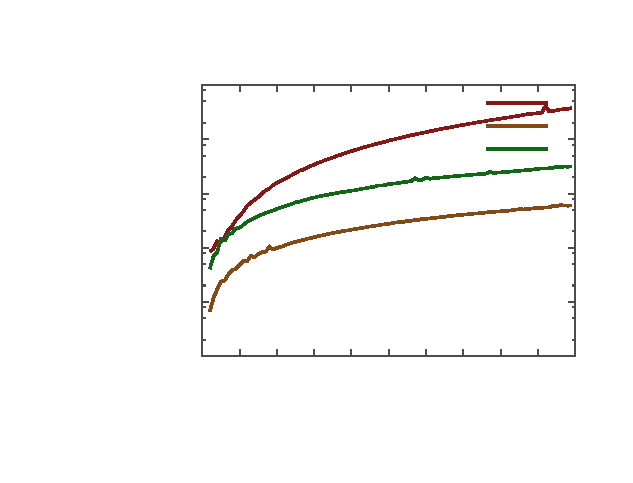
\includegraphics{./graficos/compare}}%
    \gplfronttext
  \end{picture}%
\endgroup

	}
	\end{center}
	
\end{frame}

\end{document}

